\subsection{Detektion}
SIFT gør brug af en metode kaldt Difference of Gaussian $(DoG)$, til at finde interessepunkter. $DoG$ er en skala-invariant blob detektor, og er en approksimation til en skalanormaliseret Laplacian of Gaussian $(LoG)$. $DoG$ kan udregnes, ved en subtraktion af et nærliggende skalabillede, separeret af en konstant $k$, hvor $G$ er et Gaussisk filter.
\begin{equation}
\begin{split}
DoG(x,y,\sigma) &= (G(x,y,k\sigma)-(G(x,y,\sigma))\ast I(x,y) \\
           &= L(x,y,k \sigma)-L(x,y,\sigma)
\end{split}
\label{dog}
\end{equation}
Den skalanormaliserede Laplacian of Gaussian kan opstilles som:
\begin{equation}
\begin{split}
LoG(x,y,\sigma)&=\sigma^2\nabla^2L(x,y,\sigma) \\
&= \sigma^2(L_{xx}+L{yy})
\end{split}
\end{equation}
Lowe relatere approksimeringen af $DoG$ til $LoG$, ved diffusions ligningen:
\begin{equation}
\dfrac{\partial L}{\partial \sigma} = \sigma \nabla^2L
\label{heat}
\end{equation}
Ligning \eqref{heat} kan approksimeres til:
\begin{equation}
\sigma \nabla^2L \approx \frac{G(x,y,k\sigma) - G(x,y,\sigma)}{k\sigma-\sigma}
\label{omskriv}
\end{equation}
Omskrivning af ligning \eqref{omskriv} giver:
\begin{equation}
\begin{split}
(k\sigma-\sigma)\sigma\nabla^2L &\approx L(x,y,k\sigma)-L(x,y,\sigma) \\
(k-1)\sigma^2LoG &\approx DoG
\end{split}
\end{equation}
Metoden anvender et skalarum, der deles op i oktaver, hver bestående af skalabilleder. Skalabilleder opnås ved at folde billedet iterativt med et Gaussisk filter, af stigende sigma værdi. Sigma værdien for første skalabillede, for en given oktav $l$ er dobbelt så stor som forrige: $\texttt{Start} \sigma_l = 2 \cdot \texttt{Start} \sigma_{l-1}$. Sigma værdien for et nærliggende skalabillede på samme oktav, opnås ved at multiplicere sigma værdien med en konstant $k$, dvs. $\sigma_n = \sigma_{n-1} \cdot k$. I den udførte implementering er $k=\sqrt{2}$, hvor den første sigma værdi er $1.6$. Lowe anbefaler at bruge fire oktaver, hver med syv skalabilleder. I denne implementering er der brugt fire oktaver, med fem skalabilleder pr. oktav. Metoden anvender en skalapyramide og billedet formindskes derfor til halv størrelse for hver oktav. \\ 
Når skalarummet er oprettet skal $DoG$ billederne produceres, hvilket er illustreret i figur \ref{fig:difference}(a), hvor naboliggende skalabilleder i samme oktav subtraheres. \begin{figure}[H]
    \centering
    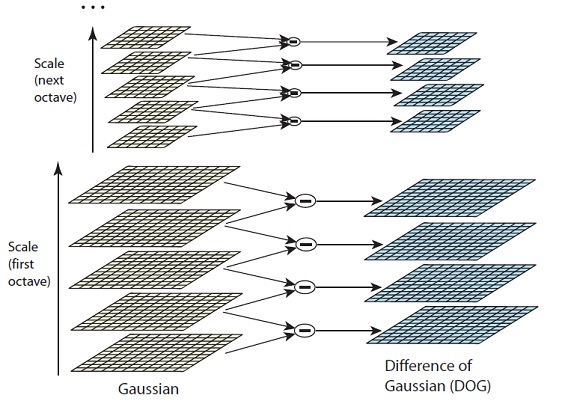
\includegraphics[width=0.90\textwidth]{fig/30.png}
     \vspace{-1em}
    \begin{center}    
       \caption{\textcolor{gray}{\footnotesize \textit{(a) Nærliggende skalabilleder for hver oktav trækkes fra og producere $DoG$ billederne. (b) I  $DoG$ billederne udvælges ekstremaer blandt 27 nabo pixels.}}}
    \label{fig:difference}
     \end{center}
     \vspace{-2.5em}
  \end{figure} \noindent    
$LoG$ svarer til sporret af hessian matricen som angiver summen af hessian matricens egenværdier. Derfor, som angivet i ligning \eqref{laplaceblob}, resultere et minima i et positivt respons og et maxima i et negativt respons. Der ønskes derved at identificere ekstremaer i $DoG$ billederne, da de vil angive forekomster af blobs. For hver pixel, sammenlignes et $3\times3\times3$ område, som vist figur \ref{fig:difference} (b). Et punkt udvælges som værende et ekstrema, hvis det er det største/mindste iblandt dens 26 naboer.
\\
\\
Når lokale ekstremaer er udvalgt fravælges dårligt lokaliserede punkter, f.eks. ekstremaer med lav kontrast, men også punkter, hvor ekstremaer ligger imellem pixels. Ligeledes bliver punkters placering fundet, med subpixel nøjagtighed. Dette gøres, ved non-maximal suppression, som foreslået af Lowe \cite{nonmaximalsuppression}:
\begin{equation}
D(x)=D+\dfrac{\partial D^T}{\partial x}x\dfrac{1}{2}x^T\dfrac{\partial^2D}{\partial x^2}x
\label{nonmax}
\end{equation}
Ovenstående kan forstås om en Taylor udvidelse af punket D.
Placeringen af ekstremaet $\hat{x}$ findes ved at tage den afledte af den ovenstående funktion ift. $x$ og sætte den til 0:
\begin{equation}
\hat{x}= \dfrac{\partial^2 D^{-1}}{\partial x^2}\dfrac{\partial D}{\partial x}
\label{xhat}
\end{equation}
Non-maximal surpression er i denne implementering anvendt anderledes end i SIFT: Lowe foreslår, at hvis et punkt er et ekstrema, som udregnet ved ligning \eqref{nonmax} og $\hat{x} > 0.5$ i en retning, skal ligning \eqref{nonmax} udregnes omkring det nye punkt og dette gentages, indtil $\hat{x} < 0.5$, eller indtil udregning er udført et max antal gange.
\\
I denne implementering bliver et punkt kun valgt, hvis $\hat{x} < 0.5$, i en given retning. Da $\xhat$ angiver en hældning i $(x, y, \sigma)$, bruges den til at frasortere punkter, det ikke er et ekstremaer. Punkters placering er ikke blevet fundet ned til sub-pixel nøjagtighed - dette blev ikke anset for en nødvendighed, da det endelige mål først var at kunne illustrere fundne korrespondancer mellem billeder (her er sub-pixel nøjagtighed ikke brugbart, da hver billedkoordinat er et naturligt heltal) - hvis der også var etableret homografier, er sub-pixel nøjagtighed strengt nødvendigt, for at få nøjagtige resultater. Implementering af non-maximal suppression som forklaret af Lowe, er næste logiske udvidelse af programmet. 
\\
Punkter med lav kontrast fjernes, ved at sætte grænseværdi, for $D(\hat{x})$:
\begin{equation}
D(\hat{x})=D+\dfrac{1}{2}\dfrac{\partial D^T}{\partial x}\hat{x}
\label{dxhat}
\end{equation}
Lowe foreslår at værdier af $D(\hat{x})$ under 0.03 fjernes. Metoden vil også have et positivt respons overfor kanter, da to meget forskellige egenværdier, vil resultere i et stærkt respons.
For at undgå dette anvendes metoder lånt fra Harris og Stephens \cite{harris}. Hessian matricen opstilles som:
\begin{equation}
\mathcal{H} =
\begin{bmatrix}
D_{xx} & D{xy} \\
D{xy} & D{yy}
\end{bmatrix}
\end{equation}
En negativ determinant angiver et saddle-point og fjernes derved. For at fjerne punkter lokaliseret på en kant beskrives forholdet imellem hessian matricens egenværdier, ved følgende ligning, hvor $r$ angiver størrelsesforholdet imellem egenværdierne:
\begin{equation}
\dfrac{tr(\mathcal{H})^2}{Det(\mathcal{H})}<\dfrac{(r+1)^2}{r}
\label{rval}
\end{equation}
En grænseværdi $r$ kan opstilles for at fjerne punkter lokaliseret på en kant. Punkter der tilfredsstiller denne grænseværdi udvælges som interessepunkter.
\subsubsection{Algoritme: Sift detektion}
\begin{enumerate}
\item[Input:] Billede $I$
\item[Output:] Interessepunkter $p \in (x,y)$
\end{enumerate}
\begin{enumerate}
\item{Skalarummet Konstrueres for de forskellige oktaver, ved iterativt at folde skalabilledet med en stigende værdi af $\sigma$: $$ L(x,y,\sigma)= G(x,y,\sigma) \ast I(x,y) $$
hvor størrelsen af billedet halveres for hver oktav.}
\item{$DoG$ billederne udregnes,ved at tage forskellen imellem skalabillederne, som i ligning \eqref{dog}.}
\item{Ekstremaer lokaliseres for hvert punkt i DOG billeder, ved at sammenligne punktet med dens 26 naboer som illustreret i figur \ref{fig:difference}.}
\item{Punkter der ikke er lokaliseret på ekstremaer, og ekstremaer med lav kontrast som i ligning \eqref{xhat} og \eqref{dxhat} afvises:
\begin{equation}
\begin{split}
\text{indikator} = 
\begin{cases}
\text{fjern}& \text{hvis } \hat{x}>0.5 \lor |D(\hat{x})|>0.03 \lor \bold{det} \mathcal{H}<0 , \\
\text{behold}& \text{ellers}. 
\end{cases}
\end{split}
\label{maxsurp}
\end{equation}
}
\item{Fjern punkter lokaliseret på en kant ved at opstille en grænseværdi $r$ og fjern punkter der ikke opfylder denne, som i ligning \eqref{rval}.}
\end{enumerate}